\chapter{Methodology\label{cha:chapter4}}
In this section, methodology used for testing hypotheses is discussed. Both primary and secondary
research methods had been used \cite{50}. Primary research was done using exploratory qualitative
interviews with help of questionnaires. Secondary research was conducted using qualitative analysis of related literature.

\section{Data Collection\label{sec:data-collection}}
Questionnaire and literature review were used to find the answers of research questions in this
paper. Questionnaire was developed using online resource \cite{51}. The
complete questionnaire is provided in  \nameref{appendix_graph}. Respondents to questionnaire were two start-
ups and one spin-off.

\section{Characteristics of Respondents of Questionnaire\label{sec:data}}
Some details on the businesses of respondents involved in questionnaire are provided in table \ref{table1}.
\begin{table} [h!]
	\centering
	\begin{tabular}{ |L{3cm}|L{3cm}|L{3cm}|L{3cm}| } 
		\hline
 	    \textbf{Name of business} & \textbf{Type of business} & \textbf{Type of work} & \textbf{Location}  \\ 
		\hline
Imsys \cite{52} & Start-up & Designs and supplies networked control solutions to OEMs in the market of Embedded Control, Telematics, Automation, and the Internet of Things  &Stockholm, Sweden \\
\hline
PTX Tech \cite{53} & Start-up & PTX presents 4D MMS  automotive solution for connected driving  & Berlin, Germany\\
\hline
Conatix \cite{54}  &Spin-off & Conatix is reinventing business research, helping companies to do market, investment and strategic research better, faster and cheaper & Berlin, Germany
\\
		\hline
	\end{tabular}
	\caption{Characteristics of respondents businesses}
	\label{table1}
\end{table}

All respondents were on the managerial level positions in their companies. Following table \ref{table2} illustrates some details on the people involved in answering questions.

\begin{table} [h!]
	\centering
	\begin{tabular}{ |c|c|L{4cm}| } 
		\hline
		  
		\textbf{Name of business} & \textbf{Role of Respondent in company} & \textbf{Years of working at current firm} \\ 
		\hline
		Imsys \cite{52} & Director Business Development & More than five years \\
		\hline
		PTX Tech \cite{53} & CEO & Less than five years \\
		\hline
		Conatix \cite{54}  & CEO & More than five year \\
		\hline
	\end{tabular}
	\caption{Characteristics of respondents of questionnaires}
	\label{table2}
\end{table}

Data collected for testing each hypothesis is presented in the following sections

\section{Data For Hypothesis 1\label{sec:data1}}
Hypothesis 1 states that transfer of resources from parent company to spin-off improves its
innovation capabilities. Since start-ups are not developed from a parent company, lack of resources in the initial stage of development affects their innovation capabilities. Questions asked for testing this hypothesis were about affects of transferring resources
from parent companies to spin-offs. Figure \ref{fig4} shows the results of primary research conducted for Hypothesis 1.
\begin{figure}[!h]
	\centering
	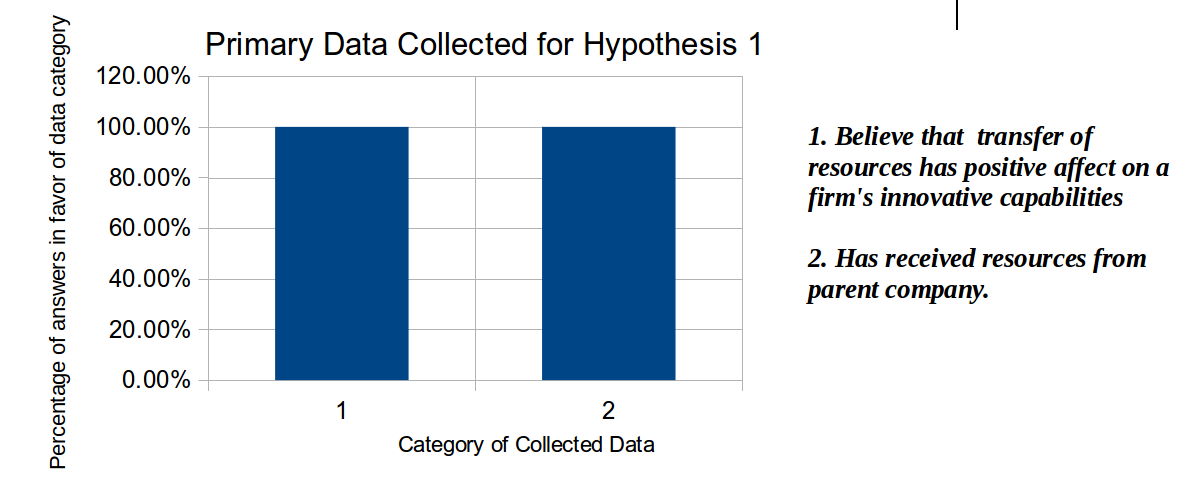
\includegraphics[width=15cm]{fig4}
	\caption{Data for Hypothesis 1}
	\label{fig4}
\end{figure}
\\
\\
Conatix CEO, David Lehrer, said the following about the resources they received
from parent company:
\\
\\
``\textbf{We received free and discounted use of office space from Humboldt University Berlin which
was valuable in the beginning, also servers and other old and used equipment from the
university}''.
\\
\\
Table \ref{table3} shows the secondary research results used for hypothesis 1.

\begin{table} [h!]
	\centering
	\begin{tabular}{ |c|L{3cm}|L{3cm}|c|L{3cm}| } 
		\hline
		\textbf{Type of resource} & \textbf{Title} & \textbf{Authors} & \textbf{Publishing Year} & \textbf{Findings} \\
		\hline
		Research Paper & Do direct or indirect relations between incumbent firms and corporate spin-offs affect the performance of spin-offs? & Majbritt Rostgaard Evald, Ann Hojbjerg Clarke, Kent Wickstrom Jensen & 2009 & Resources received by spin-
		offs through direct or indirect
		relationships with parent firms
		help them to perform better
		than independent start-ups.
		However,
		spin-offs
		with
		indirect relations to a parent
		firm perform better than spin-offs having direct relations
		\cite{35}. \\
        \hline
        
        Research Paper &Whose
        child?: 
        how
        existing
        firms foster new
        firm formation  & Sierdjan Koster  & 2006 & Transfer of resources between
        firms does not always
        guarantee the success of spin-
        off. Resources lose their
        previous designations and
        position and needs to be
        managed effectively in the
        receiving firm \cite{whose_child}. \\
        \hline
	\end{tabular}
	\caption{Secondary Research Data for Hypothesis 1}
	\label{table3}
\end{table}

\section{Data For Hypothesis 2\label{sec:data2}}
This hypothesis states that previous industry experience and managerial skills help spin-offs to
innovate better than start-ups. Questions asked to respondents for testing this hypothesis were about
previous work experience and managerial skills before joining the current organizations. Figure \ref{fig5}  shows the results of questions asked for testing Hypothesis 2.

\begin{figure}[!h]
	\centering
	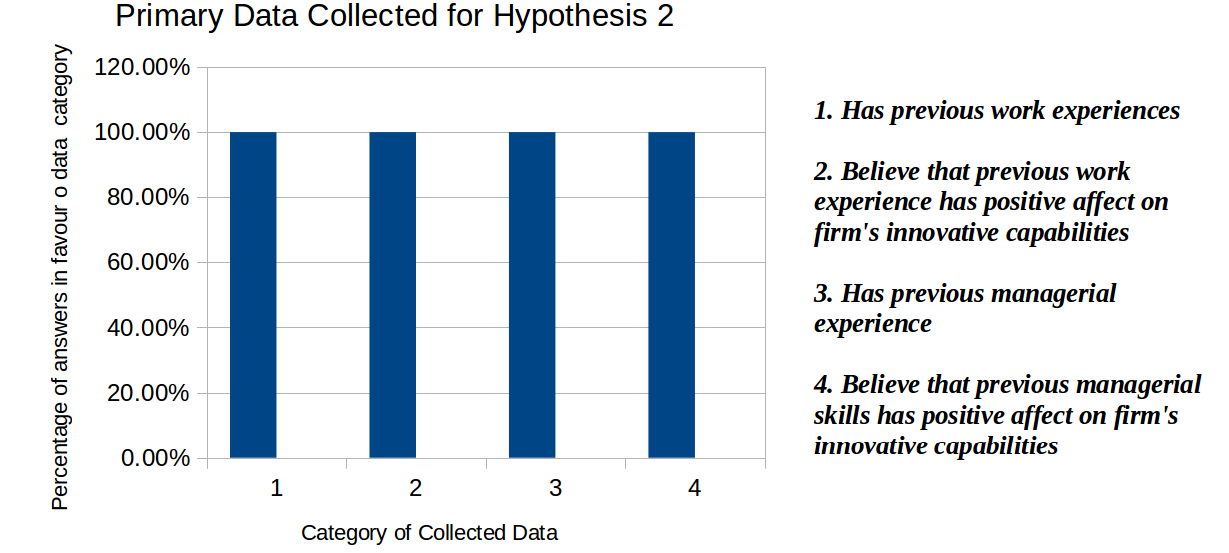
\includegraphics[width=15cm]{fig5}
	\caption{Data for Hypothesis 2}
	\label{fig5}
\end{figure}
Table \ref{table4} shows the secondary research results used for hypothesis 2.

\begin{table} [h!]
	\centering
	\begin{tabular}{ |c|L{3cm}|L{3cm}|c|L{3cm}| } 
		\hline
		\textbf{Type of resource} & \textbf{Title} & \textbf{Authors} & \textbf{Publishing Year} & \textbf{Findings} \\
		\hline
		Research paper & The effectiveness 
		of
		university knowledge
		spillovers:
		Performance
		differences
		between
		university
		spinoffs
		and
		corporate
		spinoffs &Karl Wennberg, Johan Wiklund, Mike Wright & 2011 & Previous industry experience
		in private corporations proves to be potentially more
		valuable
		for
		spin-off
		performance in than university
		experience alone \cite{55}\\
		\hline
		Book & Success Factors 
		of
		Corporat
		Spin-Off & Alexander Tübke & 2004 & Author has described transfer
		of experience as one of the
		success factors for spin-offs.
		He has mentioned that
		managerial skills are more
		valuable
		to
		progressive
		growth of a business venture
		than technical skills. He has
		given importance to different
		types
		of
		experiences
		transferred
		in
		spin-off
		development process e.g.
		market and product related,
		technical, managerial and
		leadership \cite{57} \\
		\hline
	\end{tabular}
	\caption{Secondary Research Data for Hypothesis 2}
	\label{table4}
\end{table}


\section{Data For Hypothesis 3\label{sec:data3}}
This hypothesis states that networking and relationships with clients and organizations help spin-
offs in their growth and progress. Questions asked to respondents for testing this hypothesis were
about previous networking with clients or other firms before starting their ventures. Figure \ref{fig6}
shows the results of questions asked for testing Hypothesis 3.

\begin{figure}[!h]
	\centering
	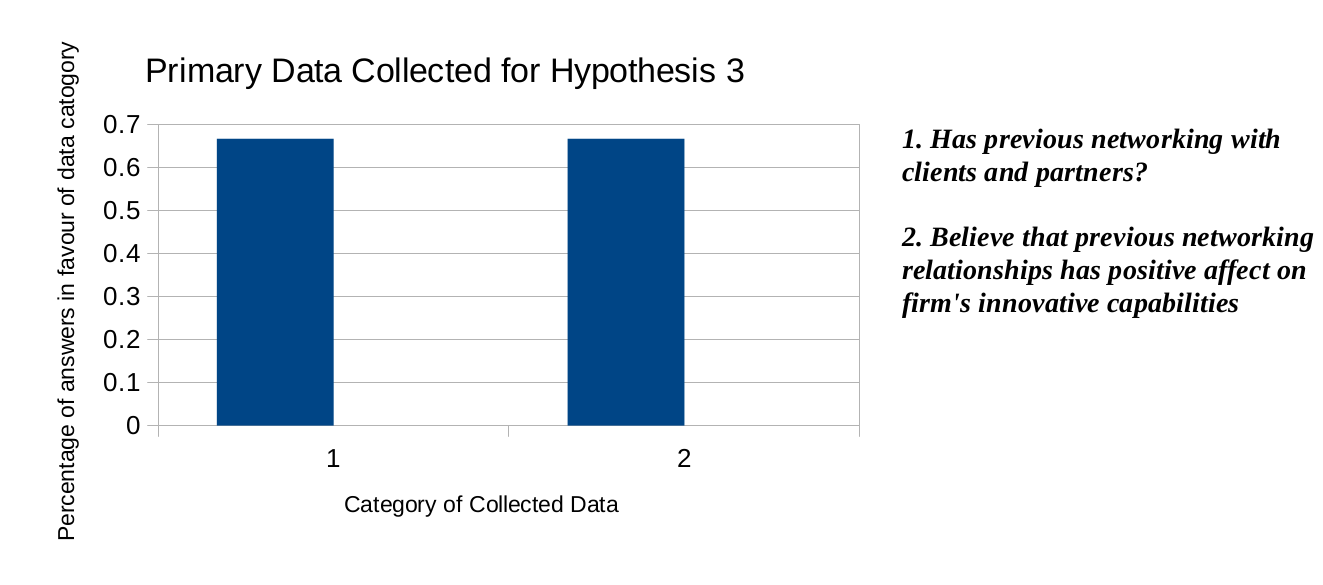
\includegraphics[width=15cm]{fig6}
	\caption{Data for Hypothesis 3}
	\label{fig6}
\end{figure}
Table \ref{table5} shows the secondary research results used for hypothesis 3.

\begin{table} [h!]
	\centering
	\begin{tabular}{ |c|L{3cm}|L{3cm}|c|L{3cm}| } 
		\hline
		\textbf{Type of resource} & \textbf{Title} & \textbf{Authors} & \textbf{Publishing Year} & \textbf{Findings} \\
		\hline
		Research Paper &Parent company 
		influence
		on
		spin-off
		performance & Tatsiana Halai & 2015 & Networking provides open
		access to potential clients,
		finances and supplies for
		product development. If the
		parent company has good
		reputation. It helps spin-offs to
		get more faith from clients
		and external relationships \cite{58}.\\
		\hline
		Research Paper & Spin-off
		firms
		and
		individual
		start-ups.
		Are
		they really
		different? &  Sierdjan Koster & 2004 & Theoretical ideas, based on
		resource theory, spin-offs
		perform better than start-ups
		based on their capabilities of
		finding ways to establish
		networks
		with
		relevant
		businesses \cite{30}. \\
		\hline
	\end{tabular}
	\caption{Secondary Research Data for Hypothesis 3}
	\label{table5}
\end{table}
\section{Data For Hypothesis 4\label{sec:data4}}
This hypothesis states that lacking the desire and passion while joining a spin-off has bad affects on
innovation development of business. Questions asked to respondents for testing this hypothesis
were about their motivations while joining the firms. Figure \ref{fig7} shows the results of
questions asked for testing Hypothesis 4.

\begin{figure}[!h]
	\centering
	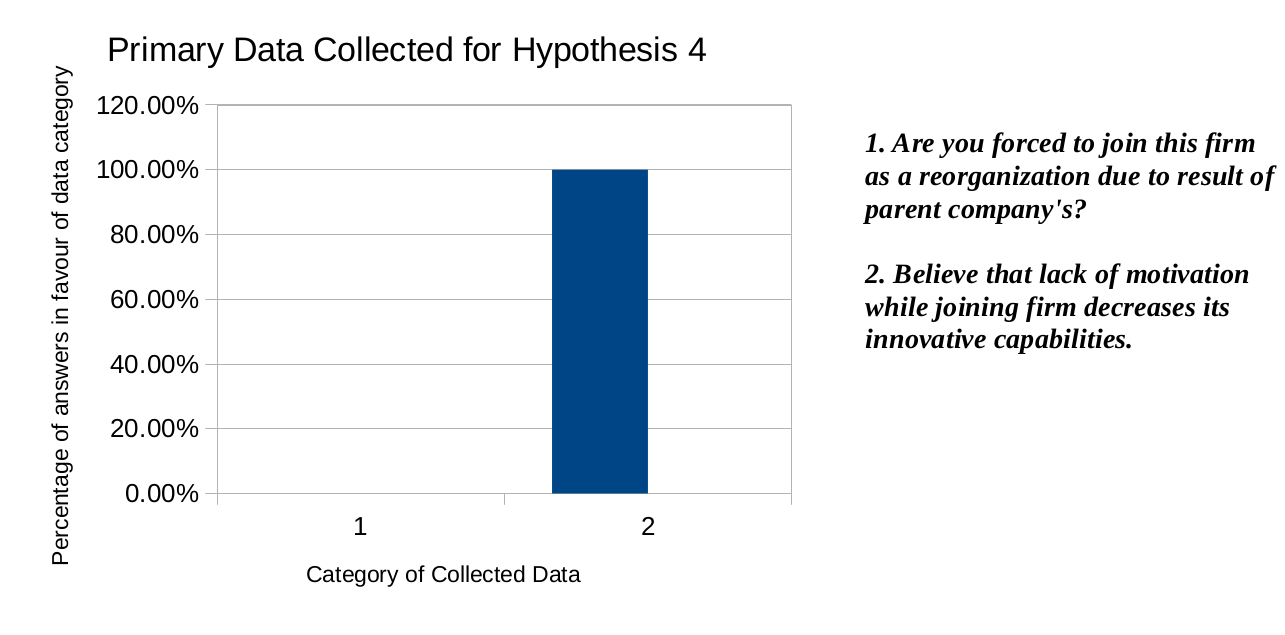
\includegraphics[width=15cm]{fig7}
	\caption{Data for Hypothesis 4}
	\label{fig7}
\end{figure}
Table \ref{table6} shows the secondary research results used for hypothesis 4.

\begin{table} [h!]
	\centering
	\begin{tabular}{ |c|L{3cm}|L{3cm}|c|L{3cm}| } 
		\hline
		\textbf{Type of resource} & \textbf{Title} & \textbf{Authors} & \textbf{Publishing Year} & \textbf{Findings} \\
		\hline
		Book & A
		Theoretical 
		and
		Empirical
		Analysis,
		with
		Special
		Reference
		to
		Education,
		Second Edition & Gary S. Becker  & 1975 & Motivation is one of the major
		factors affecting productivity
		of
		employees.
		Large
		investments on human capital
		and increase in earnings
		affects employees morale
		which
		in
		turn
		affects
		company’s growth \cite{59}. \\
		\hline
		Book & Success Factors 
		of
		Corporate 
		Spin-Off & Alexander Tübke & 2004 & Author
		has
		discussed
		motivational factor as an
		important factor affecting the
		performance of spin-off. He
		has mentioned that when
		employees are forced to join
		spin-offs against their will in
		the times of parent internal
		crisis, businesses fail badly \cite{57}.\\
		\hline
	\end{tabular}
	\caption{Secondary Research Data for Hypothesis 4}
	\label{table6}
\end{table}
